\chapter{Funciones}

\section{Las funciones y sus gráficas}

    %--------------------definición 1.1.
    \begin{tcolorbox}[colframe=white]
	\begin{def.}
	    Una función $f$ de un conjunto $D$ a un conjunto $Y$ es una regla que asigna a cada elemento $x \in D$ un solo o único elemento $f(x) \in Y$\\
	\end{def.}
    \end{tcolorbox}

    %--------------------definición 1.2.
    \begin{tcolorbox}[colframe=white]
	\begin{def.}
	    Cuando definimos una función $y = f(x)$ mediante una fórmula, y el dominio no se establece de forma explícita o se restringe por el contexto, se supondrá que el dominio será el mayor conjunto de números reales $x$ para los cuales la fórmula proporciona valores reales para $y$ , el llamado \textbf{dominio natural}.\\\\
	    Cuando el rango de una función es un subconjunto de números reales, se dice que la función tiene \textbf{valores reales (o que es real valuada)}\\
	\end{def.}
    \end{tcolorbox}

    %--------------------definición 1.3.
    \begin{tcolorbox}[colframe=white]
	\begin{def.}[Valor absoluto]
	    $f(x)=\left\{\begin{array}{rcl}
		x&si&x\geq 0\\
		\\ -x&si&x<0\\
	    \end{array} \right.$
	\end{def.}
    \end{tcolorbox}

    %--------------------definición 1.4.
    \begin{tcolorbox}[colframe=white]
	\begin{def.}
	    Sea una funcion definida en un intervalo $I$ y sean $x_1$ y $x_2$ cualesquiera dos puntos en $I$ 
	    \begin{enumerate}[\bfseries 1.]
		\item Si $f(x_2) > f(x_1)$, siempre que $x_1<x_2$ entonces se dice que $f$ es \textbf{creciente} en $I$.
		\item Si $f(x_2) < f(x_1)$, siempre que $x_1<x_2$ entonces se dice que $f$ es $\textbf{decreciente}$ en $I$.\\
	    \end{enumerate}
	\end{def.}
    \end{tcolorbox}

    %--------------------definición 1.5.
    \begin{tcolorbox}[colframe=white]
	\begin{def.}
	Una función $y=f(x)$ es una 
	    \begin{enumerate}[\bfseries 1.]
		\item Función par de $x$ si $f(-x)=f(x)$.
		\item Función impar de $x$ si $f(-x)=-f(x)$.
	    \end{enumerate}
	Para toda $x$ en el dominio de la función.\\\\
	(Los nombres par e impar provienen de las potencias de $x$).\\
	\end{def.}
    \end{tcolorbox}

    %--------------------definición 1.6.
    \begin{tcolorbox}[colframe=white]
	\begin{def.}
	    Dos variables $x$ e $y$ son \textbf{proporcionales} (una con respecto a la otra) si una siempre es un múltiplo constante de la otra; esto es, si $y=kx$ para alguna constante $k$ distinta de $0$.\\\\
	    Si la variable $y$ es proporcional al recíproco $1/x$, entonces algunas veces se dice que $y$ es \textbf{inversamente proporcional} a $x$ (puesto que $1/x$ es el inverso multiplicativo de $x$).\\

	\end{def.}
    \end{tcolorbox}


\setcounter{section}{0}
\section{Ejercicios}

\begin{enumerate}[\Large \bfseries 1.]

    %--------------------1.
    \item $f(x)=1+x^2$ \\\\
	Respuesta.-\; Al evaluar $1+x^2$ vemos que $x$ se cumple para todos los reales, por lo tanto $f_D=\lbrace x /; \forall \; x \in \mathbb{R} \rbrace$. Luego el rango viene dado por $f_R=\lbrace y=f(x) / y \geq 1 \rbrace$\\\\

    %--------------------2.
    \item $f(x)=1-\sqrt{x}$\\\\
       Respuesta.-\; El dominio viene dado por $f_D=\lbrace x / x \geq 0 \rbrace$. Y el rango viene dado por $f_R = \lbrace y = f(x) / y \leq 1 \rbrace$.\\\\

    %--------------------3.
    \item $F(x)=\sqrt{5x + 10}$\\\\
	Respuesta.-\; Sea $5x + 10 \geq 0$ ya que una raíz par no puede ser no negativo, entonces $x \geq 2$, por lo tanto el dominio viene dado por $f_D=\lbrace x / x \geq -2 \rbrace$. Luego el rango viene dado por $f_R = \lbrace y=f(x) / y \geq 0 \rbrace$.\\\\

    %--------------------4.
    \item $g(x)=\sqrt{x^2 - 3x}$\\\\
	Respuesta.-\; De igual forma al anterior ejercicio, evaluaremos $x^2 - 3x \geq 0$, de donde $x(x-3)\geq 0$, por lo tanto el dominio es $f_D=\lbrace x/\leq x \leq 0 \cup x \geq 3 \rbrace$. Luego el rango viene definido por $f_R=\lbrace y=f(x) / y \geq 0 \rbrace$.\\\\

    %--------------------5.
    \item $f(t)=\dfrac{4}{3-t}$ \\\\
	Respuesta.-\; Sabemos que no se puede dividir un número por $0$. Por lo tanto para hallar el dominio de la función debemos evaluar $3-t=0$, de donde $t=3$, así $f_D=\lbrace t / t\neq 3\rbrace$. Luego el rango viene dado por $f_R=\lbrace y=f(x) / y\neq 0\rbrace$.\\\\

    %--------------------6.
    \item $G(t)=\dfrac{2}{t^2 - 16}$ \\\\
	Respuesta.-\; De igual forma al anterior ejercicio evaluamos $t^2 - 16 = 0$, de donde $(t - 4)(t + 4)=0$, por lo tanto el dominio de la función viene dado por $f_D=\lbrace t / t \neq 4 \land t \neq -4 \rbrace$. Luego el rango viene dado por $f_R=\lbrace y=f(x) / 0 < y \leq - \dfrac{1}{8} \rbrace$ ya que al despejar $x$ nos queda  $x=\sqrt{\dfrac{2}{y} + 16}$ de donde se debe evaluar por un lado $\dfrac{2}{y}$ y por otro $\dfrac{2}{y} - 16 \geq 0$.\\\\

    En los ejercicios $7$ y $8$ ¿Cuál de las gráficas representa la gráfica de una función de $x$? ¿Cuáles no representan a funciones de $x$? Dé razones que apoyen sus respuestas.\\\\

    %--------------------7.
    \item El inciso $a.$ no es una función ya que no cumple con la prueba de la recta vertical ya una función sólo puede tener un valor $f(x)$ para cada $x$ en su dominio. Y el inciso $b.$ no representa la gráfica de una función.\\\\

    %--------------------8.
    \item Los incisos $a.$ y $b.$ no representan a funciones de $x$. El único que no representa una gráfica de una función es el inciso $b.$\\\\

    Determinación de fórmulas para funciones.\\\\

    %--------------------9.
    \item Exprese el área y el perímetro de un triángulo equilátero como una función del lado $x$ del triángulo.\\\\
	Respuesta.-\; El área se representa por $f(x)=\dfrac{\sqrt{3}a^2}{4}$ y el perímetro por $f(x)=3x$\\\\

    %--------------------10.
    \item Exprese la longitud del lado de un cuadrado como una función de la longitud $d$ de la diagonal del cuadrado. Exprese el área como una función de la longitud de la diagonal.\\\\
	Respuesta.-\; La longitud del lado de un cuadrado como función de longitud esta dado por $d=\sqrt{2a^2}$. El área es expresado por $A=\dfrac{d^2}{2}$\\\\

    %--------------------11.
    \item Exprese la longitud del lado de um cubo como una función de la longitud de la diagonal $d$ del cubo. Exprese el área de la superficie y el volumen del cubo como una función de la longitud de la diagonal.\\\\
	Respuesta-.\; La expresión de la longitud del lado del cubo como función de la longitud de la diagonal $d$ del cubo es  $$ L(d) = (\sqrt{2}/2)\cdot d $$ 
	Las expresiones del área de la superficie y el volumen del cubo como función de la longitud de la diagonal $d$ del cubo son:
	$$A(d) = 3\cdot d² \quad    y \quad  V(d) = (\sqrt{2}/4)\cdot d³$$

    %--------------------12.
    \item Un punto $P$ en el primer cuadrante pertenece a la gráfica de la función $f(x)=\sqrt{x}$. Exprese las coordenadas de $P$ como funciones de la pendiente de la recta que une a $P$ con el origen.\\\\
	Respuesta.-\; Sea el punto en el origen $(0,0)$ y el punto $P$ tenga las coordenadas $(z,z^{'})$. Sabemos que una recta viene definido por $f(x)=ax+b$ entonces formando un sistema de ecuaciones tenemos:
	$$0=0x + b \quad y \quad z^{'} = az + b$$
	Luego $z^{'}=az$ de donde $a=\dfrac{z^{'}}{z}$, y así nos queda la función  
	$$f(x)=\dfrac{z^{'}}{z} x$$\\\\

    %--------------------13.
    \item Considere el punto $(x,y)$ que está en la gráfica de la recta $2x + 4y = 5$. Sea $L$ la distancia del punto $(x, y)$ al origen $(0, 0)$. Escriba $L$ como función de $x$.\\\\
	Respuesta.-\; Dado $(x,y) \in 2x+4y=5 ; (0,0)$ entonces $$x=\dfrac{5-4y}{2} \qquad \dfrac{5-2x}{4}$$
	Luego $L=\sqrt{(y-0)^2+(x-0)^2} = \sqrt{y^2 + \left( \dfrac{5-4y}{2}\right)}=\sqrt{y^2 + \dfrac{25+40y+16y^2}{4}}=\sqrt{\dfrac{4y^2}{4} + \dfrac{25 - 40y + 16y^2}{4}} = \dfrac{1}{2} \sqrt{20y^2 + 40y + 25}$\\\\
 
    %--------------------14.
    \item Considere el punto $(x, y)$ que está en la gráfica de $y = \sqrt{x - 3}$. Sea $L$ la distancia entre los puntos $(x,y)$ y $(4,0)$. Escriba $L$ como función de $y$.\\\\
	Respuesta.-\; $y=\sqrt{x-3}, (x,y)\in y=\sqrt{x-3}$ entonces calculamos la distancia entre $y=\sqrt{x-3}$ y $(4,0)$.\\
	$$y^2=x-3 \Longrightarrow x=y^2 + 3 \quad y \quad y=\sqrt{x-3}$$ 
	Así $L=\sqrt{(y-o)^2 + (x-y)^2} = \sqrt{y^2 + (y^2 + 3)^2} = \sqrt{y^2 + y^4 + 6y^2 + 9} = \sqrt{y^4+7y^2+9}$\\\\

    Las funciones y sus gráficas.\\\\
    En los ejercicios $15$ al $20$, determine el dominio y grafique las funciones\\\\

    %--------------------15.
    \item $f(x)=5-2x$\\\\
	Respuesta.-\; El dominio esta dado para todos los reales $x$.
	\begin{center}
	    \begin{tikzpicture}[scale=1,draw opacity = 0.6]
		% abscisa y ordenada
		\tkzInit[xmax= 3,xmin=-2,ymax=5,ymin=-1]
		\tiny\tkzLabelXY[opacity=0.6,step=1, orig=false]
		% etiqueta x, f(x)
		\tkzDrawX[opacity=0.6,label=x,right=0.3]
		\tkzDrawY[opacity=0.6,label=f(x),below = -0.6]
		%dominio y función
		\draw [domain=-1:3,thick,gray] plot(\x,{5-2*\x});
		\tkzText[opacity=0.6,above](2,3){\tiny $f(x)=5-2x$}
	    \end{tikzpicture}
	\end{center}
	\vspace{.5cm}

    %--------------------16.
    \item $f(x)=1-2x-x^2$\\\\ 
	Respuesta.-\; El dominio viene dado para todo real $x$ positivo.
	\begin{center}
	    \begin{tikzpicture}[scale=1,draw opacity = 0.6]
		% abscisa y ordenada
		\tkzInit[xmax= 2,xmin=-3,ymax=3,ymin=-3]
		\tiny\tkzLabelXY[opacity=0.6,step=1, orig=false]
		% etiqueta x, f(x)
		\tkzDrawX[opacity=0.6,label=x,right=0.3]
		\tkzDrawY[opacity=0.6,label=f(x),below = -0.6]
		%dominio y función
		\draw [domain=-3:1,thick,gray] plot(\x,{1-2*\x - \x*\x});
		\tkzText[opacity=0.6,above](1.3,1){\tiny $f(x)=1-2x-x^2$}
	    \end{tikzpicture}
	\end{center}
	\vspace{.5cm}

    %--------------------17.
    \item $g(x)=\sqrt{|x|}$\\\\ 
	Respuesta.-\; El dominio de la función es para $x \in \mathbb{R}$
	\begin{center}
	    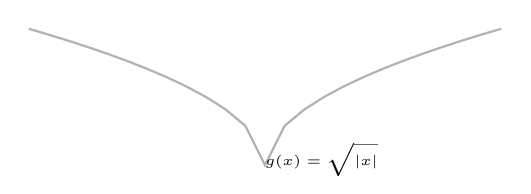
\begin{tikzpicture}[scale=1,draw opacity = 0.6]
		% abscisa y ordenada
		\tkzInit[xmax= 3,xmin=-3,ymax=3,ymin=0]
		\tiny\tkzLabelXY[opacity=0.6,step=1, orig=false]
		% etiqueta x, f(x)
		\tkzDrawX[opacity=0.6,label=x,right=0.3]
		\tkzDrawY[opacity=0.6,label=f(x),below = -0.6]
		%dominio y función
		\draw [domain=-3:3,thick,gray] plot(\x,{abs(\x)^(1/2)});
		\tkzText[opacity=0.6,above](1,1.7){\tiny $g(x)=\sqrt{|x|}$}
	    \end{tikzpicture}
	\end{center}
	\vspace{.5cm}

    %--------------------18.
    \item $g(x) = \sqrt{-x}$\\\\
	Respuesta.-\; El dominio de la función se cumple para los números reales negativos.   
	\begin{center}
	    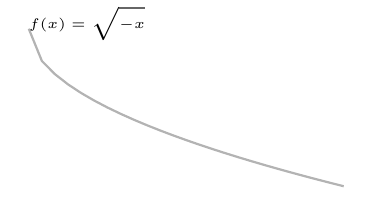
\begin{tikzpicture}[scale=1,draw opacity = 0.6]
		% abscisa y ordenada
		\tkzInit[xmax= 4,xmin=-1,ymax=1,ymin=-2]
		\tiny\tkzLabelXY[opacity=0.6,step=1, orig=false]
		% etiqueta x, f(x)
		\tkzDrawX[opacity=0.6,label=x,right=0.3]
		\tkzDrawY[opacity=0.6,label=f(x),below = -0.6]
		%dominio y función
		\draw [domain=0:4,thick,gray] plot(\x,{-\x^(1/2)});
		\tkzText[opacity=0.6,above](2,-1){\tiny $f(x)=\sqrt{-x}$}
	    \end{tikzpicture}
	\end{center}
	\vspace{.5cm}

    %--------------------19.
    \item $F(t)=t/|t|$\\\\
	Respuesta.-\; El dominio viene dado para todo número real menos el $0$. 
	\begin{center}
	    \begin{tikzpicture}[scale=1,draw opacity = 0.6]
		% abscisa y ordenada
		\tkzInit[xmax= 3,xmin=-3,ymax=2,ymin=-2]
		\tiny\tkzLabelXY[opacity=0.6,step=1, orig=false]
		% etiqueta x, f(x)
		\tkzDrawX[opacity=0.6,label=x,right=0.3]
		\tkzDrawY[opacity=0.6,label=f(x),below = -0.6]
		%dominio y función
		\draw [domain=.1:3,thick,gray] plot(\x,{\x/abs(\x)});
		\draw [domain=-3:-.1,thick,gray] plot(\x,{\x/abs(\x)});
		\tkzText[opacity=0.6,above](1,1){\tiny $F(t)=t/|t|$}
	    \end{tikzpicture}
	\end{center}
	\vspace{.5cm}

    %--------------------20.
    \item $G(t)=1/|t|$\\\\
	Respuesta.-\; El dominio se cumple para todo número real menos el $0$.
	\begin{center}
	    \begin{tikzpicture}[scale=1,draw opacity = 0.6]
		% abscisa y ordenada
		\tkzInit[xmax= 3,xmin=-3,ymax=5,ymin=0]
		\tiny\tkzLabelXY[opacity=0.6,step=1, orig=false]
		% etiqueta x, f(x)
		\tkzDrawX[opacity=0.6,label=x,right=0.3]
		\tkzDrawY[opacity=0.6,label=f(x),below = -0.6]
		%dominio y función
		\draw [domain=.2:3,thick,gray] plot(\x,{1/abs(\x)});
		\draw [domain=-3:-.2,thick,gray] plot(\x,{1/abs(\x)});
		\tkzText[opacity=0.6,above](2,2){\tiny $G(t)=1/|t|$}
	    \end{tikzpicture}
	\end{center}
	\vspace{.5cm}

    %--------------------21
    \item Determine el dominio de $y=\dfrac{x+3}{4-\sqrt{x^2-9}}$\\\\
	Respuesta.-\; Si $y=f(x)$ entonces el dominio esta dado por $D_f=\lbrace x / x\geq 3 \land x \neq 4 \rbrace$ \\\\

    %--------------------22.
    \item Determine el rango de $y=2+\dfrac{x^2}{x^2+4}$.\\\\
	Respuesta.-\; Si $y=f(x)$ entonces el rango viene dado para todo $y=f(x)$ tal que $y\geq 2$\\\\

    %--------------------23.
    \item Grafique las siguientes ecuaciones y explique por qué no son gráficas de funciones de $x$.\\\\
    
    \begin{enumerate}[\bfseries a.]
	
	%----------a.
	\item $|y|=x$\\\\
	    Respuesta.-\; No es una función de $x$ ya que $ \sqrt{y^2}=x \Longrightarrow y^2=x^2 \Longrightarrow \pm y = \pm x$\\\\

	%----------b.
	\item $y^2 = x^2$\\\\
	    Respuesta.-\; Por el anterior problema $23a.$\\\\
	
    \end{enumerate}

    %--------------------24.
    \item Grafique las siguientes ecuaciones y explique por qué no son gráficas de funciones de $x$\\\\

    \begin{enumerate}[\bfseries a.]

	%----------a.
	\item $|x|+|y|=1$\\\\
	    Respuesta.-\; Ya que $|y|=1 - |x| \Longrightarrow \sqrt{y^2} = 1 - |x| \Longrightarrow y^2 = (1-|x|)^2 \Longrightarrow \pm y= |1-|x||$\\\\

	%----------b.
	\item $|x+y|=1$\\\\
	Respuesta.-\;  Ya que $\sqrt{(x+y)^2}=1 \Longrightarrow (x+y)^2 = 1 \Longrightarrow x^2 + 2xy + y^2 = 1 \Longrightarrow y^2 = 1 - 2xy - x^2 \Longrightarrow \pm y = \sqrt{1-2xy-x^2}$\\\\
    \end{enumerate}

    Funciones definidas por partes\\\\
    En los ejercicios 25 a 28, grafique las funciones:\\\\

    %--------------------25.
    \item $f(x) = \left\{ \begin{array}{cc}
		    x,&0\leq x \leq 1\\
		    \\ 2-x,&1<x\leq 2 \\
		    \end{array} \right.$
	\begin{center}
	    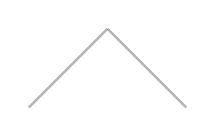
\begin{tikzpicture}[scale=1,draw opacity = 0.6]
		% abscisa y ordenada
		\tkzInit[xmax= 3,xmin=-1,ymax=2,ymin=0]
		\tiny\tkzLabelXY[opacity=0.6,step=1, orig=false]
		% etiqueta x, f(x)
		\tkzDrawX[opacity=0.6,label=x,right=0.3]
		\tkzDrawY[opacity=0.6,label=f(x),below = -0.6]
		%dominio y función
		\draw [domain=0:1,thick,gray] plot(\x,{\x});
		\draw [domain=1:2,thick,gray] plot(\x,{2-\x});
	    \end{tikzpicture}
	\end{center}
	\vspace{.5cm}
    
    %--------------------26.
    \item $g(x) = \left\{ \begin{array}{cc}
		    1-x,&0\leq x \leq 1\\
		    \\ 2-x,&1<x\leq 2 \\
		    \end{array} \right.$
	\begin{center}
	    
\begin{tikzpicture}[scale=1,draw opacity = 0.6]
		% abscisa y ordenada
		\tkzInit[xmax= 3,xmin=-1,ymax=2,ymin=0]
		\tiny\tkzLabelXY[opacity=0.6,step=1, orig=false]
		% etiqueta x, f(x)
		\tkzDrawX[opacity=0.6,label=x,right=0.3]
		\tkzDrawY[opacity=0.6,label=f(x),below = -0.6]
		%dominio y función
		\draw [domain=0:1,thick,gray] plot(\x,{1-\x});
		\draw [domain=1:2,thick,gray] plot(\x,{2-\x});
	    \end{tikzpicture}
	\end{center}
	\vspace{.5cm}
    
    %--------------------27.
    \item $F(x) = \left\{ \begin{array}{cc}
		    4-x^2,&\leq 1 \\
		    \\ x^2 + 2x,& x>1 \\
		    \end{array} \right.$
	\begin{center}
	    \begin{tikzpicture}[scale=1,draw opacity = 0.6]
		% abscisa y ordenada
		\tkzInit[xmax= 3,xmin=-3,ymax=8,ymin=0]
		\tiny\tkzLabelXY[opacity=0.6,step=1, orig=false]
		% etiqueta x, f(x)
		\tkzDrawX[opacity=0.6,label=x,right=0.3]
		\tkzDrawY[opacity=0.6,label=f(x),below = -0.6]
		%dominio y función
		\draw [domain=-2:1,thick,gray] plot(\x,{4-\x*\x});
		\draw [domain=1:2,thick,gray] plot(\x,{\x*\x + 2*\x});
	    \end{tikzpicture}
	\end{center}
	\vspace{.5cm}

    %--------------------28.
    \item $G(x) = \left\{ \begin{array}{cc}
		    1/x,&x<0\\
		    \\ x, & 0\leq x \\
		    \end{array} \right.$
	\begin{center}
	    \begin{tikzpicture}[scale=1,draw opacity = 0.6]
		% abscisa y ordenada
		\tkzInit[xmax= 3,xmin=-4,ymax=2,ymin=-8]
		\tiny\tkzLabelXY[opacity=0.6,step=1, orig=false]
		% etiqueta x, f(x)
		\tkzDrawX[opacity=0.6,label=x,right=0.3]
		\tkzDrawY[opacity=0.6,label=f(x),below = -0.6]
		%dominio y función
		\draw [domain=-3:0,thick,gray] plot(\x,{1*\x^(-1)});
		\draw [domain=0:2,thick,gray] plot(\x,{\x});
	    \end{tikzpicture}
	\end{center}
	\vspace{.5cm}

    Determine una fórmula para cada función graficada en los ejercicios $29$ a $32$\\\\

    %--------------------29
    \item 
    \begin{enumerate}[\bfseries a.]
	
	%----------a.
	\item  Sea $f(x)=ax+b$ entonces $0=b$ y $1=a+b$ luego $a=1$ por lo tanto $f(x)=x$. Por otro lado $1=a+b$ y $0=2a+2 \Longrightarrow a=-1$ de donde se tiene $f(x^{'})=-x+2$ así nos queda la función:
	$$f(x) = \left\{\begin{array}{r c l}
		x&si&0\leq x \leq 1\\
		\\ x+2&si&1\leq x \leq 2 \\
	    \end{array}\right.$$\\\\

	%----------b.
	\item Está definida por $$f(x)=\left\{\begin{array}{rcl} 
				    2&si&0\leq x < 1 \; o \; 2 \leq x < 3\\
				    \\  0&si& 1\leq x < 2 \; ó \; 3\leq x \leq 4\\
				    \end{array}\right.$$\\\\

    %--------------------30.
    \item 

    \end{enumerate}

\end{enumerate}
